\section{Key Terms (N-grams) and their Frequency \& Sentiment}
In this section, the trends in climate change discussions on Reddit are explored by analyzing the frequency and sentiment of key terms over time. Using the \emph{Counter} class from Python's \emph{collections} module, the most frequently mentioned unigrams and bigrams related to climate change were identified. Initially, the most frequent 100 uni- and bigrams were calculated. However, due to the non-preprocessed nature of the dataset, many of these frequent terms did not offer much meaningful information (e.g., terms like "http", "just", "know", "like", "make need", "don think", "don believe", "org wiki", "feel like"). Therefore, several relevant terms were manually hand-picked to focus on in the analysis. This approach provides clearer insights into the shifting focus of climate-related conversations and the associated sentiments expressed by Reddit users.

\subsection{Unigrams}
\subsubsection{Frequency}
\begin{figure}[h]
    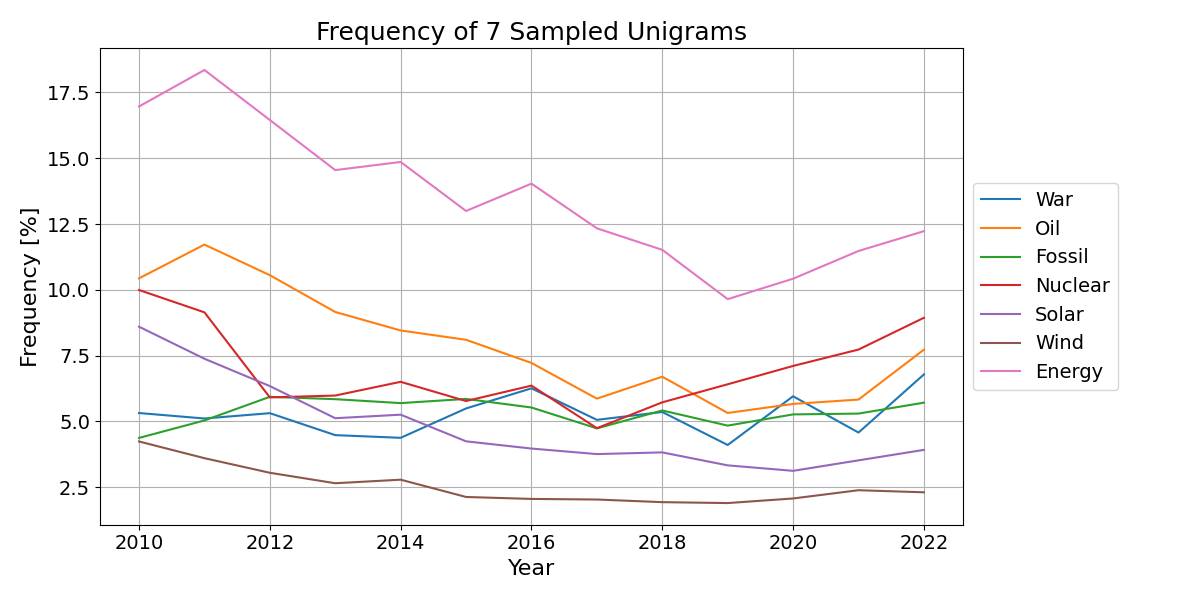
\includegraphics[width=\textwidth]{images/topic_details/ngram/frequency_per_topic_7Unigram.png}
    \caption{Frequency distribution of unigrams war, oil, fossil, nuclear, solar, wind, and energy}
    \label{fig:frequency_unigrams}
\end{figure}
The plot in Figure \ref{fig:frequency_unigrams} presents the frequency of seven selected unigrams over time. These unigrams include "war", "oil", "fossil", "nuclear", "solar", "wind", and "energy". The frequency is represented as a percentage of total unigram occurrences per year. The selected key terms, except for \emph{war}, are all related to energy. Energy is a crucial factor in the context of climate change because the production and consumption of energy are major sources of greenhouse gas emissions. Changing to renewable energy sources like solar and wind, and reducing dependence on fossil fuels such as oil and nuclear energy, are essential strategies for mitigating climate change and achieving sustainable development. These energy-related discussions reflect the importance of energy policy and technology in addressing climate change challenges.

The term \emph{war} is included in the analysis to highlight its relevance to climate change discussions especially when it comes to its sentiment. Conflicts and geopolitical tensions can have significant impacts on energy resources and climate policies, making it an important topic within the broader context of climate change discourse. Also, this indicates that discussions about war and its impact on climate change have been a consistent topic of interest. Debates about the environmental impacts of wars, such as resource consumption and destruction of ecosystems, contribute to this trend \cite{hsiang2014climate}.

Both \emph{oil} and \emph{fossil} terms show different trends. The frequency of discussions around \emph{oil} shows a decrease over the years, reflecting a growing awareness and shift towards renewable energy sources and away from fossil fuels. On the other hand, the term \emph{fossil}, represented by the green line, remains relatively stable with a slight increase. This stability and slight increase might indicate ongoing discussions about fossil fuels, especially in the context of debates around energy policies and climate change mitigation strategies. Major events, such as the Paris Agreement in 2015, which aimed to limit global warming by reducing greenhouse gas emissions, played a significant role in shifting public and policy focus towards cleaner energy alternatives \cite{unfccc2015paris}.

The frequency of \emph{nuclear} discussions has a noticeable drop post-2011, aligning with the Fukushima Daiichi nuclear disaster. This incident raised global concerns about the safety of nuclear energy, leading to more cautious and often negative discussions around this energy source \cite{WNA2012}. The decrease is also associated with several countries re-evaluating their nuclear policies and energy strategies as a result of the disaster.

\begin{figure}[h]
    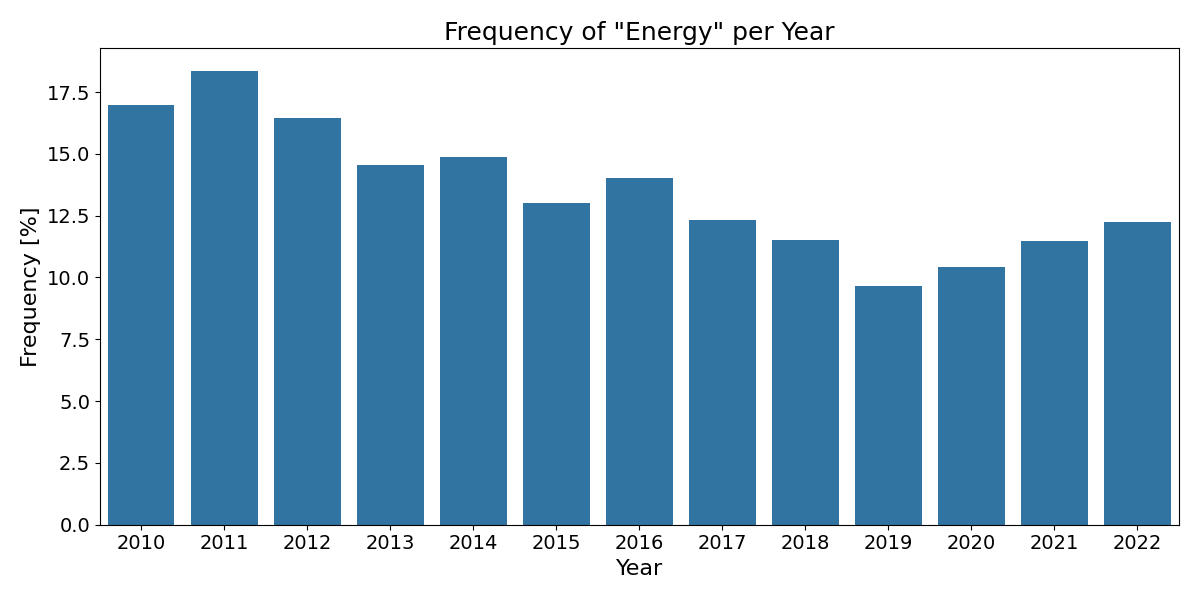
\includegraphics[width=\textwidth]{images/topic_details/ngram/frequency_bar_energy.png}
    \caption{Detailed Frequency Distribution of \emph{energy}}
    \label{fig:frequency_energy}
\end{figure}

Terms like \emph{solar} and \emph{wind} show a decreasing trend over the years. The frequency of discussions around \emph{wind} energy, represented by the brown line, has decreased from approximately 4\% to 2.5\%. Similarly, the frequency of \emph{solar} energy discussions, represented by the purple line, has dropped from around 9\% to 4\%. This decreasing trend could be attributed to the initial rise in discussions and interest when these technologies were newer and perceived as more revolutionary. As these renewable energy sources have become more established and integrated into mainstream energy discussions, the novelty may have worn off, leading to fewer mentions relative to other topics. However, the ongoing interest and investment in renewable energy technologies are driven by government policies and international commitments to reduce greenhouse gas emissions, such as the European Union's Renewable Energy Directive and various national incentives for renewable energy projects \cite{irena2018roadmap}.

The term \emph{energy} with a detailed bar plot in Figure \ref{fig:frequency_energy} shows the frequency of the term \emph{energy} per year. The term has been consistently discussed, with a notable peak in 2011. This rise likely corresponds to increased discourse surrounding energy policies and the push for sustainable energy solutions during that period. The global focus on energy efficiency and the transition to renewable energy sources could have driven these discussions. The increased focus on energy in 2011 may also be attributed to policy discussions and implementations following the Fukushima disaster, emphasizing the need for safer and cleaner energy alternatives \cite{iea2011policies}.

\subsubsection{Sentiment}
\begin{figure}[h]
    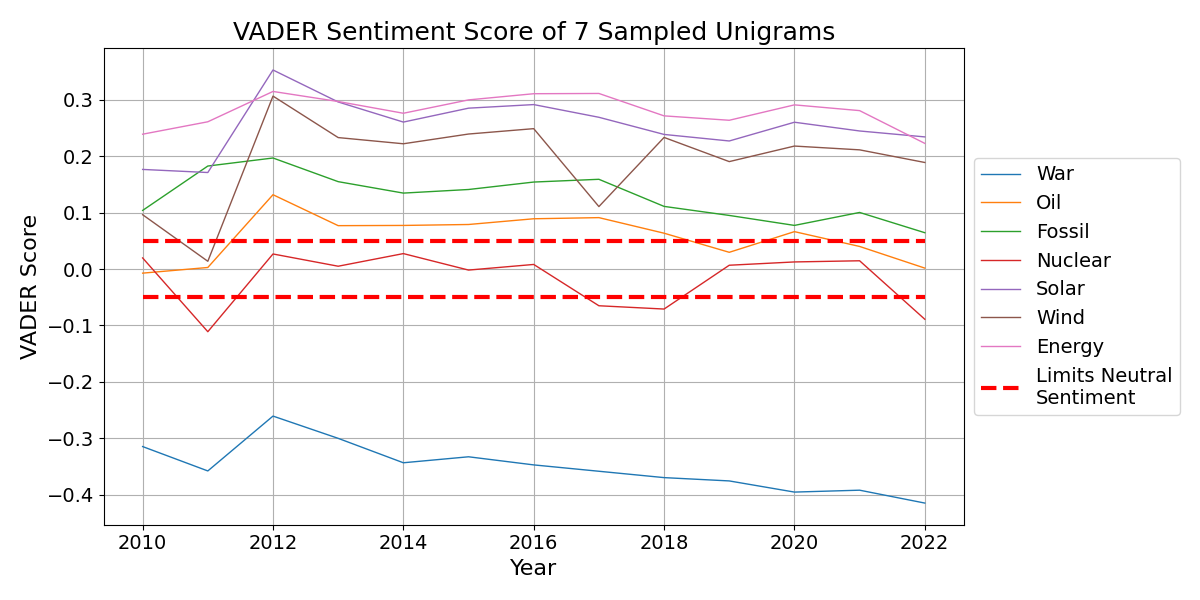
\includegraphics[width=\textwidth]{images/topic_details/ngram/sentiment_per_topic_7Unigram.png}
    \caption{Sentiment Scores of Unigrams \emph{war}, \emph{oil}, \emph{fossil}, \emph{nuclear}, \emph{solar}, \emph{wind} and \emph{energy}}
    \label{fig:sentiment_unigrams}
\end{figure}
The sentiment plot in Figure \ref{fig:sentiment_unigrams} displays the VADER sentiment scores for the same set of unigrams. Sentiment scores range from -1 (very negative) to 1 (very positive), with the red dashed lines indicating the limits for neutral sentiment.

\emph{War} consistently holds a negative sentiment, reflecting the unfavorable impacts and concerns associated with war on the environment and society. On the other hand, \emph{energy} shows the highest positive sentiment overall, indicating optimistic discussions about energy solutions and innovations. The positive sentiment around \emph{energy} suggests that discussions are often framed in a constructive context, focusing on advancements and potential solutions for climate change.

\emph{Nuclear} experiences its lowest sentiment in 2011, reflecting public doubts about nuclear energy's safety and environmental risks. This is a direct consequence of the Fukushima disaster, which led to a rise in negative perceptions about nuclear energy globally \cite{WNA2012}. Despite this, \emph{nuclear} sentiment scores are generally within the neutral range, except for the drops in 2011, 2017, 2018, and 2022. The relatively neutral sentiment in other years suggests that discussions about nuclear energy include both its risks and its potential as a low-carbon energy source.

Conversely, \emph{solar} and \emph{wind} maintain generally positive sentiments, highlighting favorable perceptions and the potential of these renewable energy sources in mitigating climate change. This positive outlook is likely driven by the increasing efficiency, decreasing costs, and widespread adoption of solar and wind technologies \cite{irena2018roadmap}. Even \emph{oil} despite its association with fossil fuels, shows a positive sentiment in most years, reflecting discussions around technological advancements in reducing emissions or the economic importance of oil.

Several factors could contribute to \emph{oil} maintaining a higher sentiment than \emph{nuclear}. First, oil has historically been a critical driver of economic growth, providing energy for transportation, industry, and households \cite{CAVALCANTI2013475}. Discussions about oil often highlight its economic benefits and the technological advancements aimed at reducing its environmental impact, such as carbon capture and storage (CCS) and cleaner extraction methods (IEA, 2019).
Second, the oil industry has invested significantly in public relations and marketing to maintain a positive image, emphasizing the role of oil in modern society and efforts to transition to cleaner technologies \cite{ExxonMobil2021}. This could lead to a more favorable perception of oil compared to nuclear energy, which has struggled with public relations, particularly after high-profile accidents like Chernobyl and Fukushima.
Overall, while \emph{nuclear} energy is perceived neutrally to negatively, \emph{oil} consistently maintains a higher sentiment, except for 2010. This trend might be due to ongoing discussions about the economic benefits of oil and advancements in cleaner technologies for its use, which can sometimes overshadow the negative aspects related to its environmental impact.

\subsection{Bigrams}
\subsubsection{Frequency}
\begin{figure}[h]
    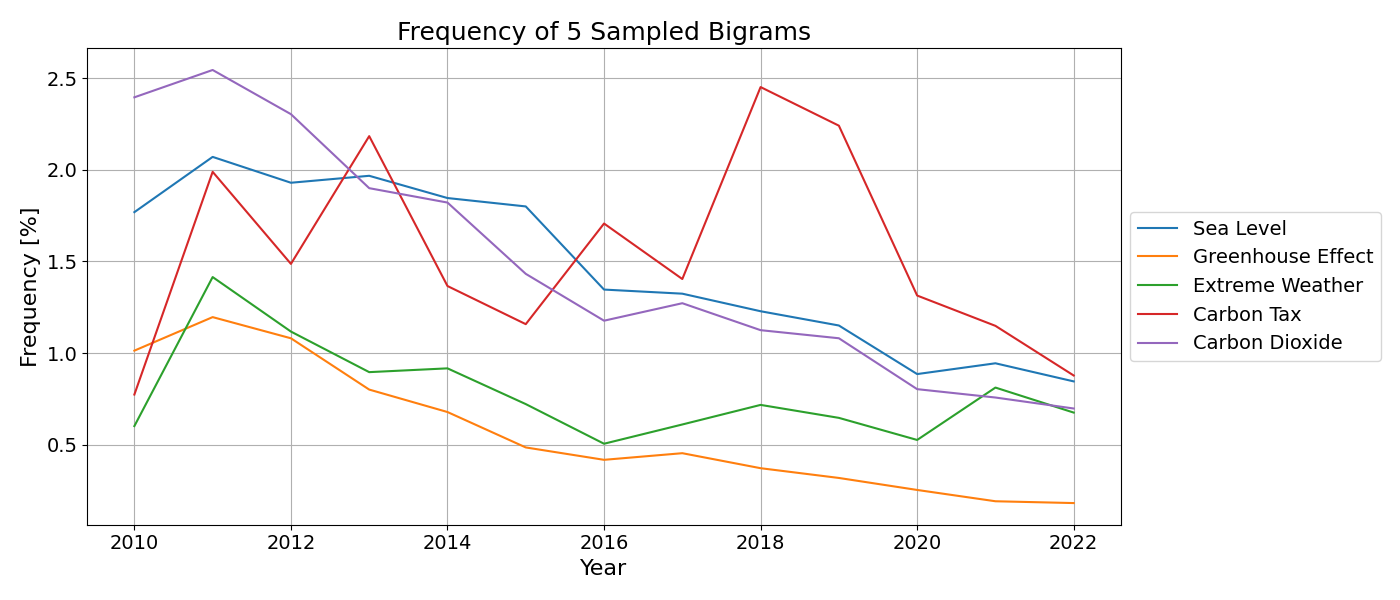
\includegraphics[width=\textwidth]{images/topic_details/ngram/frequency_per_topic_5Bigram.png}
    \caption{Frequency Distribution of Bigrams \emph{sea level}, \emph{greenhouse effect}, \emph{extreme weather}, \emph{carbon tax} and \emph{carbon dioxide}}
    \label{fig:frequency_bigrams}
\end{figure}

The plot shown in Figure \ref{fig:frequency_bigrams} provides the frequency of five selected bigrams: sea level, greenhouse effect, \emph{extreme weather}, carbon tax and \emph{carbon dioxide}

The term \emph{carbon tax} peaks in frequency in 2011, 2013, 2018, and 2019. These peaks correspond to periods of intense policy discussions and implementations related to carbon pricing mechanisms. For example, in 2011, Australia introduced a significant carbon tax aimed at reducing carbon emissions, leading to extensive debates and discussions \cite{worldbank2018carbon}. In 2013, British Columbia's carbon tax was widely discussed due to its innovative approach and effectiveness in reducing emissions \cite{murray2015bc}. The peaks in 2018 and 2019 align with renewed global discussions on carbon pricing as a critical tool for meeting the Paris Agreement targets, with several countries either implementing or considering carbon tax policies during these years \cite{worldbank2018carbon}.
The term \emph{carbon tax} also highlights the complexities and challenges associated with implementing such policies. These discussions often center around economic impacts, public acceptance, and the effectiveness of carbon taxes in reducing emissions. The repeated peaks suggest that the topic remains disputed and relevant, reflecting ongoing policy evaluations and adjustments in various regions. The fluctuation in frequency underscores the dynamic nature of climate policy debates and the role of public discourse in shaping these policies.

The decreasing trend of \emph{greenhouse effect} suggests that the term may be getting replaced by more specific and complex discussions around climate change impacts and solutions. This could reflect a shift in discourse from basic concepts to more complex and targeted climate change issues, such as carbon footprints, renewable energy technologies, and specific environmental policies \cite{ipcc2014impacts}. The decreasing use of \emph{greenhouse effect} may indicate that the public and policymakers are moving beyond basic education about climate change to more action-oriented discussions.
Furthermore, the reduction in the use of \emph{greenhouse effect} might also be attributed to the evolution of climate change communication strategies. As public understanding of climate change has increased, there has been a corresponding shift towards discussing mitigation and adaptation strategies in more specific terms. This shift is essential for driving effective policy measures and encouraging practical solutions to tackle climate change. It also reflects the broader trend in environmental communication, where the focus is increasingly on actionable steps rather than basic concepts.

Another significant observation is the decrease in the frequency of \emph{sea level} and \emph{carbon dioxide}. The frequency of \emph{sea level} discussions has significantly dropped over the years. This might be due to the increasing focus on more immediate and impactful climate issues such as renewable energy sources and policy measures like carbon taxes. Although sea level rise remains a critical aspect of climate change, the public discourse may have shifted towards addressing the causes of climate change more directly, such as carbon emissions and energy use \cite{nasa2020,nasa2020co2}.

The term \emph{carbon dioxide} shows a noticeable decrease in frequency, dropping from approximately 2.4\% to 0.7\%. This drop could indicate a shift in the language used to discuss emissions and climate change. As climate science and policy discussions have evolved, terms like \emph{carbon footprint} or \emph{greenhouse gases} might be more frequently used, reflecting a broader understanding and more sophisticated discourse about emissions and their impacts \cite{unep2019}. The shift from \emph{carbon dioxide} to other terms might also suggest a more integrated approach to discussing various greenhouse gases collectively, rather than focusing on a single component.

\subsubsection{Sentiment}
\begin{figure}[h]
    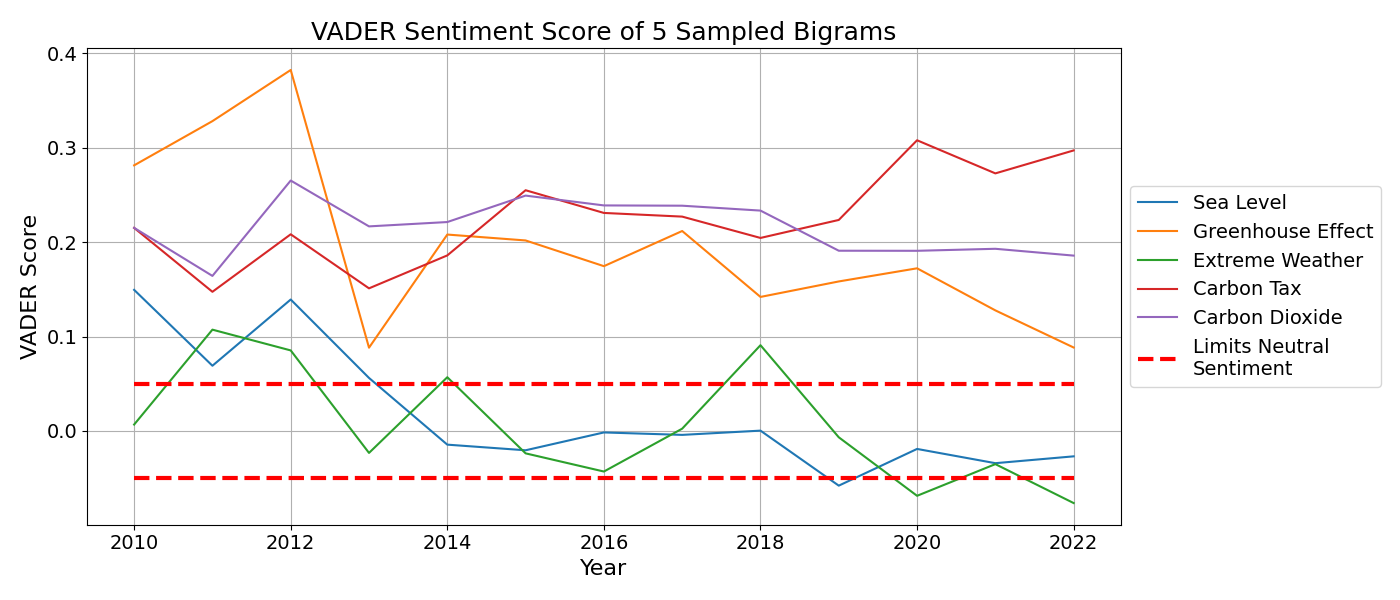
\includegraphics[width=\textwidth]{images/topic_details/ngram/sentiment_per_topic_5Bigram.png}
    \caption{Sentiment Scores of Bigrams \emph{sea level}, \emph{greenhouse effect}, \emph{extreme weather}, \emph{carbon tax} and \emph{carbon dioxide}}
    \label{fig:sentiment_bigrams}
\end{figure}
The sentiment plot in Figure \ref{fig:sentiment_bigrams} displays the VADER sentiment scores for the same set of unigrams. Sentiment scores range from -1 (very negative) to 1 (very positive), with the red dashed lines indicating the limits for neutral sentiment.

\emph{Carbon tax} shows a slight but steady increase in sentiment over the years, starting around 0.2 and rising to 0.3. This positive trend likely reflects growing support for carbon pricing as an effective way to reduce greenhouse gas emissions. The introduction of carbon taxes in various regions and their success in lowering emissions might have contributed to this positive sentiment \cite{murray2015bc}.

\emph{Greenhouse effect} reached its highest sentiment in 2012 but then dropped significantly from 0.38 to 0.09 in 2013. The peak in 2012 might be linked to increased awareness of climate change impacts and global climate agreements. However, the sharp drop in 2013 could be due to a shift in discussions towards more specific and actionable climate issues, reducing the prominence of the \emph{greenhouse effect} in public conversations \cite{ipcc2014impacts}.

\emph{Extreme weather} has fluctuating sentiments, with positive sentiment scores in 2011, 2012, 2014, and 2018. The peak in 2018 likely corresponds to heightened awareness and discussions about extreme weather events, which may have been framed positively due to increased persistence and preparedness measures. Notable extreme weather events in 2018 include a record number of wildfires in California, such as the devastating Camp Fire, which highlighted the importance of disaster preparedness and persistence \cite{CalFire2018}.
In contrast, the years 2020 and 2022 show a drop in sentiment for \emph{extreme weather} into the negative range. This shift could be attributed to the significant and devastating weather events that occurred during these years, such as the Australian bushfires (Black Summer) in 2020, which caused widespread destruction and raised global concern about climate change's impact on weather patterns \cite{BBC2020}. Additionally, the severe flooding in Pakistan in 2022 displaced millions of people and caused extensive damage, emphasizing the negative impacts of climate change on vulnerable regions \cite{cordaid2022}.

\emph{Sea level} does not show a stable sentiment over the years. It changes from positive sentiment class years (2010 - 2015) to a neutral period, with 2019 standing out with a negative sentiment class. The negative sentiment in 2019 could be linked to several alarming reports and events regarding sea level rise. For example, a report by the United Nations in 2019 highlighted the accelerated pace of sea level rise and its potential catastrophic impacts on coastal communities worldwide \cite{UN2019}.

\emph{Carbon dioxide}, on the other hand, shows a relatively stable sentiment over the years, reflecting ongoing discussions about its role in climate change without significant fluctuations in public perception.

Overall, the sentiment analysis of selected bigrams offers a detailed understanding of climate change conversations on Reddit. The positive sentiment around terms like \emph{carbon tax} suggests optimism towards policy measures for climate change mitigation. The fluctuating sentiment for \emph{extreme weather} highlights the emotional impact of these events and the varying public perceptions they generate. Similarly, the changing sentiment towards \emph{sea level} underscores the growing concern about the observable impacts of climate change on the environment.

In summary, this analysis provides valuable insights into the public's perception of different climate-related topics over time. Recognizing the positive and negative sentiments associated with these terms can help in framing climate change communication strategies to promote constructive and informed discussions.

\section{From n-grams to Entities: Enhancing Text Analysis with SpaCy}
In the previous sections, the analysis was conducted using unigrams and bigrams to identify key terms and trends in climate change discussions on Reddit. While this approach provides valuable insights, it has certain limitations. N-grams are simple sequences of words and do not account for context, variations in terminology, or the semantic relationships between terms. This is where named entity recognition (NER) using advanced natural language processing (NLP) tools like SpaCy becomes essential.

Named entities are real-world objects, such as people, organizations, locations, and events, that can be identified and categorized in text. Using SpaCy, a powerful and efficient NLP library, allows for a more sophisticated analysis by detecting these entities within the text. Here are several reasons why moving from bare n-grams to entities is advantageous:

\begin{enumerate}
    \item \textbf{Contextual Understanding:} Entities provide context that n-grams often lack. For example, the unigram \emph{Trump} could refer to different contexts depending on the discussion. By recognizing \emph{Donald Trump} as an entity, the analysis can focus specifically on mentions of the person rather than the word "Trump" in other contexts.
    \item \textbf{Normalization of Variations:} NER helps in normalizing variations of the same entity. Different ways of referring to the same entity (e.g., "U.S.A.", "United States", "America") can be identified and consolidated into a single entity, improving the accuracy and clarity of the analysis.
    \item \textbf{Reduced Noise:} N-grams often include common words that do not carry significant meaning on their own (e.g., "http", "know", "like"). Entity recognition filters out such noise by focusing on specific, meaningful entities, leading to a more focused and relevant analysis.
    \item \textbf{Sentiment Analysis:} By associating sentiments with entities rather than standalone words or phrases, the sentiment analysis becomes more accurate. For instance, analyzing the sentiment towards \emph{climate change} as an entity is more informative than analyzing the sentiment of the individual words "climate" and "change".
    \item \textbf{Enhanced Trend Detection:} Entities allow for tracking more meaningful trends over time. For instance, tracking the mentions and sentiment of specific organizations like \emph{Greenpeace} or events like \emph{Paris Agreement} provides deeper insights into public discourse and shifts in opinion.
    \item \textbf{Interconnected Insights:} Entities can be linked to other entities, providing insights into relationships and co-occurrences within the text. For example, analyzing how often \emph{climate change} is mentioned alongside \emph{renewable energy} can reveal interconnected discussions and thematic linkages.
\end{enumerate}

Making use of SpaCy and its entity recognition capabilities into the analysis allows for a richer, more detailed understanding of the discussions around climate change on Reddit. This transition from basic n-gram analysis to entity-based analysis marks a significant improvement in extracting valuable insights and making data-driven conclusions.

\section{SpaCy's Named Entities and their Frequency \& Sentiment}
In this section, the analysis moves from simple n-gram counting to a more advanced entity recognition approach using spaCy's Entity Recognizer. This method allows for a deeper understanding of the entities mentioned in climate change discussions on Reddit and their interconnections. The focus is on the entities labeled as PERSON, GPE (Geopolitical Entity), ORG (Organization), NORP (Nationalities or Religious or Political Groups), LOC (Location), and EVENT. SpaCy's entity recognition forms the basis of our analysis. Some entities have been normalized by their text (\emph{Trump} becomes \emph{Donald Trump}) or corrected by their label, while entities that were not recognized were not modified.

\subsection{An Example of Entities and their Interconnections}
Before exploring the network analysis, it is helpful to understand how entities are identified and categorized within the comments. The provided example in Figure \ref{fig:displacy} is a snippet of a Reddit comment from 2017, which has one of the lowest sentiments. This snippet displays the output of spaCy's named entity recognition (NER) tool and its visualization retrieved by displaCy, highlighting various entities within the text.

Entities are labeled as follows:
\begin{itemize}
    \item \textbf{PERSON:} Individuals mentioned, such as \emph{Sarkeesian}, \emph{Trump}, and \emph{Clinton}.
    \item \textbf{NORP:} Nationalities, religious, or political groups, such as \emph{Arab-American}, \emph{American}, and \emph{Muslim}.
\end{itemize}

\begin{figure}[h]
    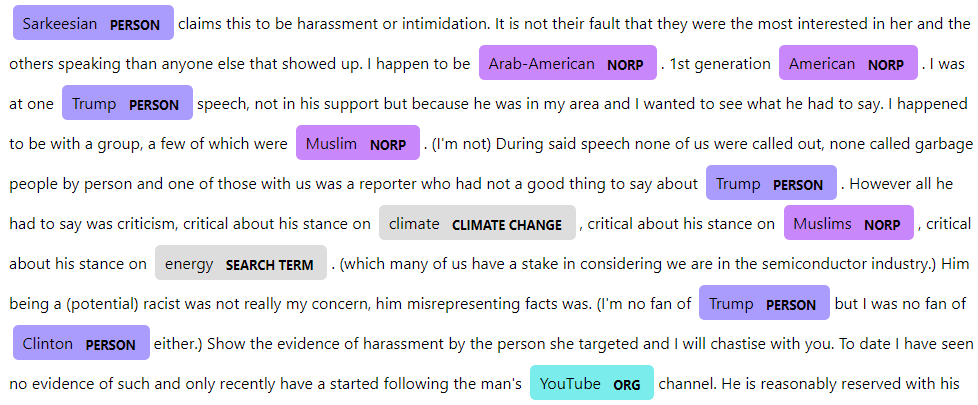
\includegraphics[width=\textwidth]{images/topic_details/entities/displaCy.PNG}
    \caption{Snippet of a Reddit Comment from 2017 with Entities Identified by SpaCy and Entity Label Corrections, Featuring the Unigram and Search Term \emph{energy}\protect\footnotemark}
    \label{fig:displacy}
\end{figure}
\footnotetext{\emph{Trump} was labeled as ORG by spaCy.}
Additionally, specific terms relevant to our analysis, like \emph{climate change} and \emph{energy}, are customized and highlighted in gray to emphasize their significance for this snippet.

Examining the interconnections within this snippet:
\begin{itemize}
    \item \emph{Sarkeesian} (PERSON) and \emph{Trump} (PERSON) are both prominent figures whose actions and statements can significantly influence public opinion. The mention of Trump is connected to a speech, which is noted for its critical stance.
    \item \emph{Arab-American} (NORP) and \emph{Muslim} (NORP) reflect the identities of individuals in the context of Trump's (PERSON) speech, highlighting the intersection of climate discourse with social and political identities.
    \item \emph{American} (NORP) is used to describe a broader national identity, often linked to discussions about national policies and leadership.
    \item \emph{Clinton} (PERSON) appears in contrast to \emph{Trump} (PERSON), showing the political divide and differences in stances on climate issues.
\end{itemize}

This method of entity recognition allows for a more structured analysis of text data, providing insights into how different entities are interconnected and discussed over time. It sets the stage for our detailed examination of network graphs, where the relationships and sentiments associated with these entities will be explored to understand the broader narrative and sentiment trends in climate change discussions.

\subsection{Network Analysis}
To visualize the relationships between these entities, network graphs have been created for each year. These graphs not only show the connections between entities but also indicate the average sentiment score associated with each entity. The sentiment scores, ranging from -1 (very negative) to 1 (very positive), are averaged from the sentiments of the comments in which the entities are mentioned.

It is important to note that many of the entities identified in these discussions are not directly related to major climate change topics. Instead, they highlight the heavy intersection between climate change and global politics. This emphasizes that climate change is not an isolated topic; it intersects with almost all major global issues today. Analyzing climate change discourse without considering the geopolitical context would provide an incomplete picture.

The decision to focus on election years for this analysis is driven by the significant impact that political leadership and election effects have on climate change policies and discourse. Election years often bring heightened attention to political figures, policies, and national priorities, making them critical periods for understanding shifts in public sentiment and discussion topics. Political campaigns, debates, and media coverage during these times can greatly influence public opinion and the prioritization of climate change in the national agenda. By examining the network of entities during election years, we can gain insights into how political dynamics shape climate change discourse and identify key influencers and sentiments that drive public conversations.

\subsubsection{2012 Network Analysis}
\begin{figure}[h]
    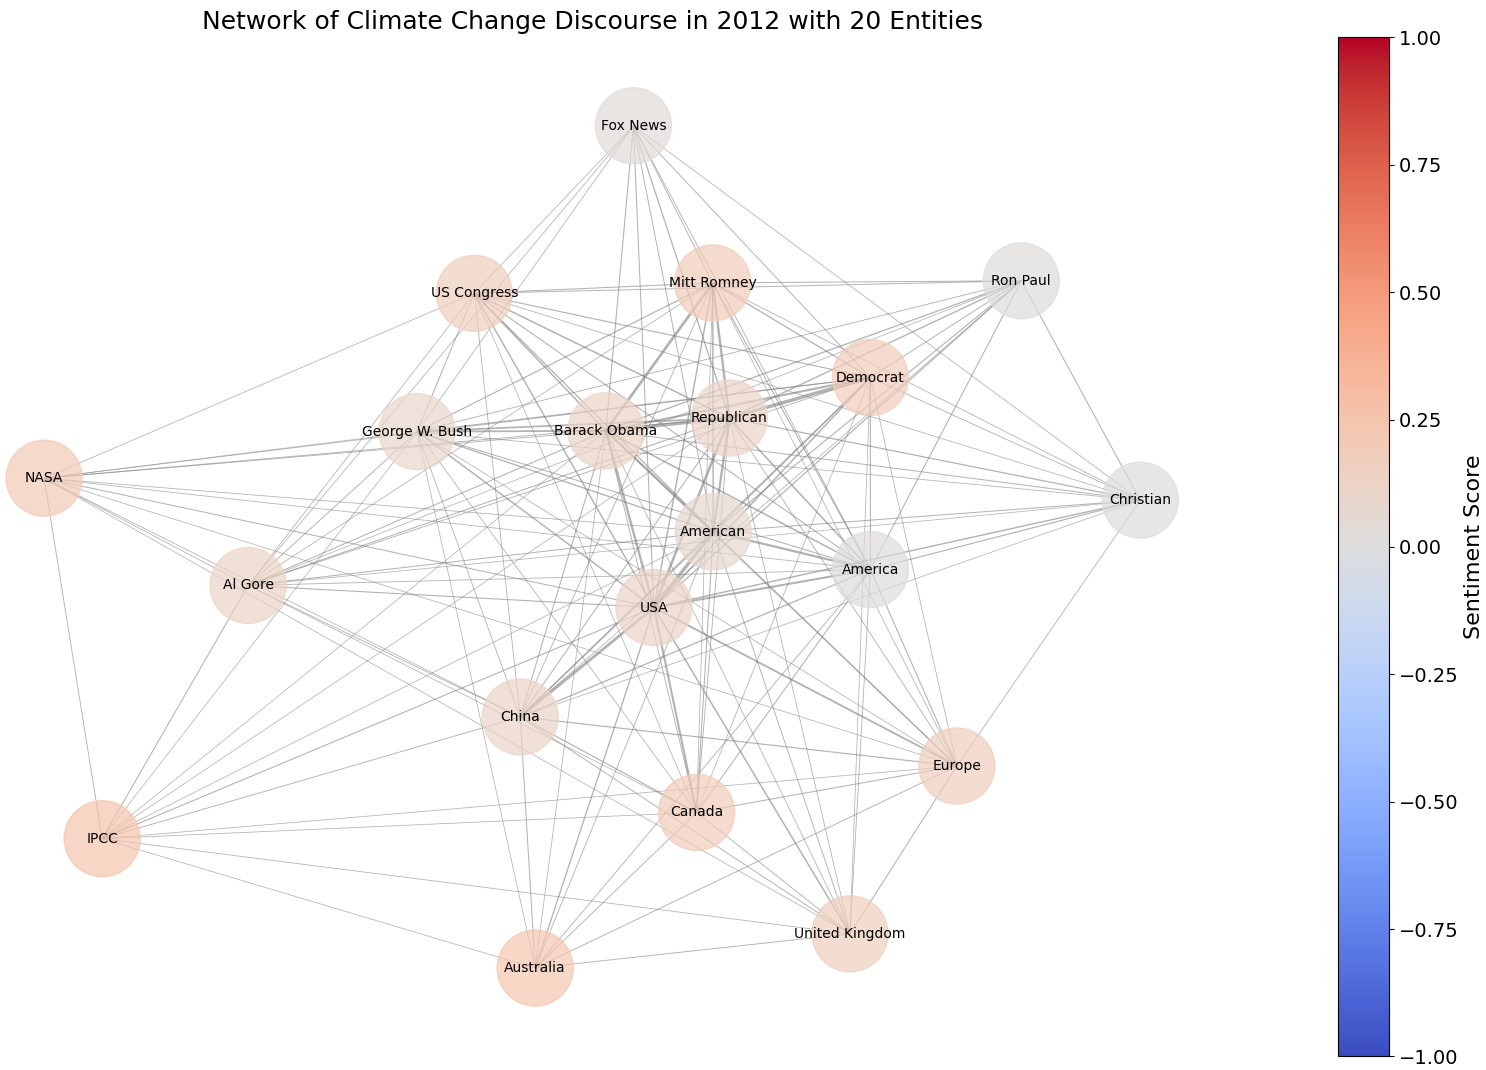
\includegraphics[width=\textwidth]{images/topic_details/entities/network_analysis_top20_2012_spring.png}
    \caption{Network of 20 Most Frequent Entities and their Sentiment in 2012}
    \label{fig:network_2012}
\end{figure}
The network graph for 2012 in Figure \ref{fig:network_2012} highlights a US-centric discourse around climate change. Key entities include political figures like Barack Obama and George W. Bush, organizations such as the US Congress and NASA, and geopolitical entities like the USA and China. The sentiment scores are predominantly neutral to slightly positive, reflecting a period of political stability and ongoing environmental initiatives.

\begin{description}
    \item[Overall Sentiment:] The 2012 graph shows the highest overall sentiment among the years analyzed, which is also visible in Figure \ref{fig:mean_sentiment}. This could be attributed to the general optimism surrounding Obama's re-election campaign, which emphasized clean energy and environmental protection \cite{obama2013climate}.
    \item[Democratic and Republican Candidates:] The key figures in the election were \emph{Barack Obama} (Democrat) and \emph{Mitt Romney} (Republican), with Obama winning re-election.
    \item[IPCC Inclusion:] The Intergovernmental Panel on Climate Change (\emph{IPCC}) is included due to its influential role in climate science and policy. The release of its assessment reports often drives significant discourse on climate change \cite{IPCC2014}. For example, the IPCC's Fourth Assessment Report, released in 2007, and the Special Report on Renewable Energy Sources and Climate Change Mitigation, released in 2011, were significant in shaping global climate policy.
    \item[Christian Entity:] The mention of \emph{Christian} with the lowest sentiment (still within the neutral sentiment class) could reflect discussions around the intersection of religion and climate change, possibly touching on topics like environmental leadership or skepticism about climate science within some religious communities. Prominent Christian figures or groups during the 2012 election year, such as Evangelical leaders and organizations like the Evangelical Environmental Network, often engage in debates on climate change from a religious perspective \cite{Veldman2019}.
\end{description}

\subsubsection{2016 Network Analysis}
\begin{figure}[h]
    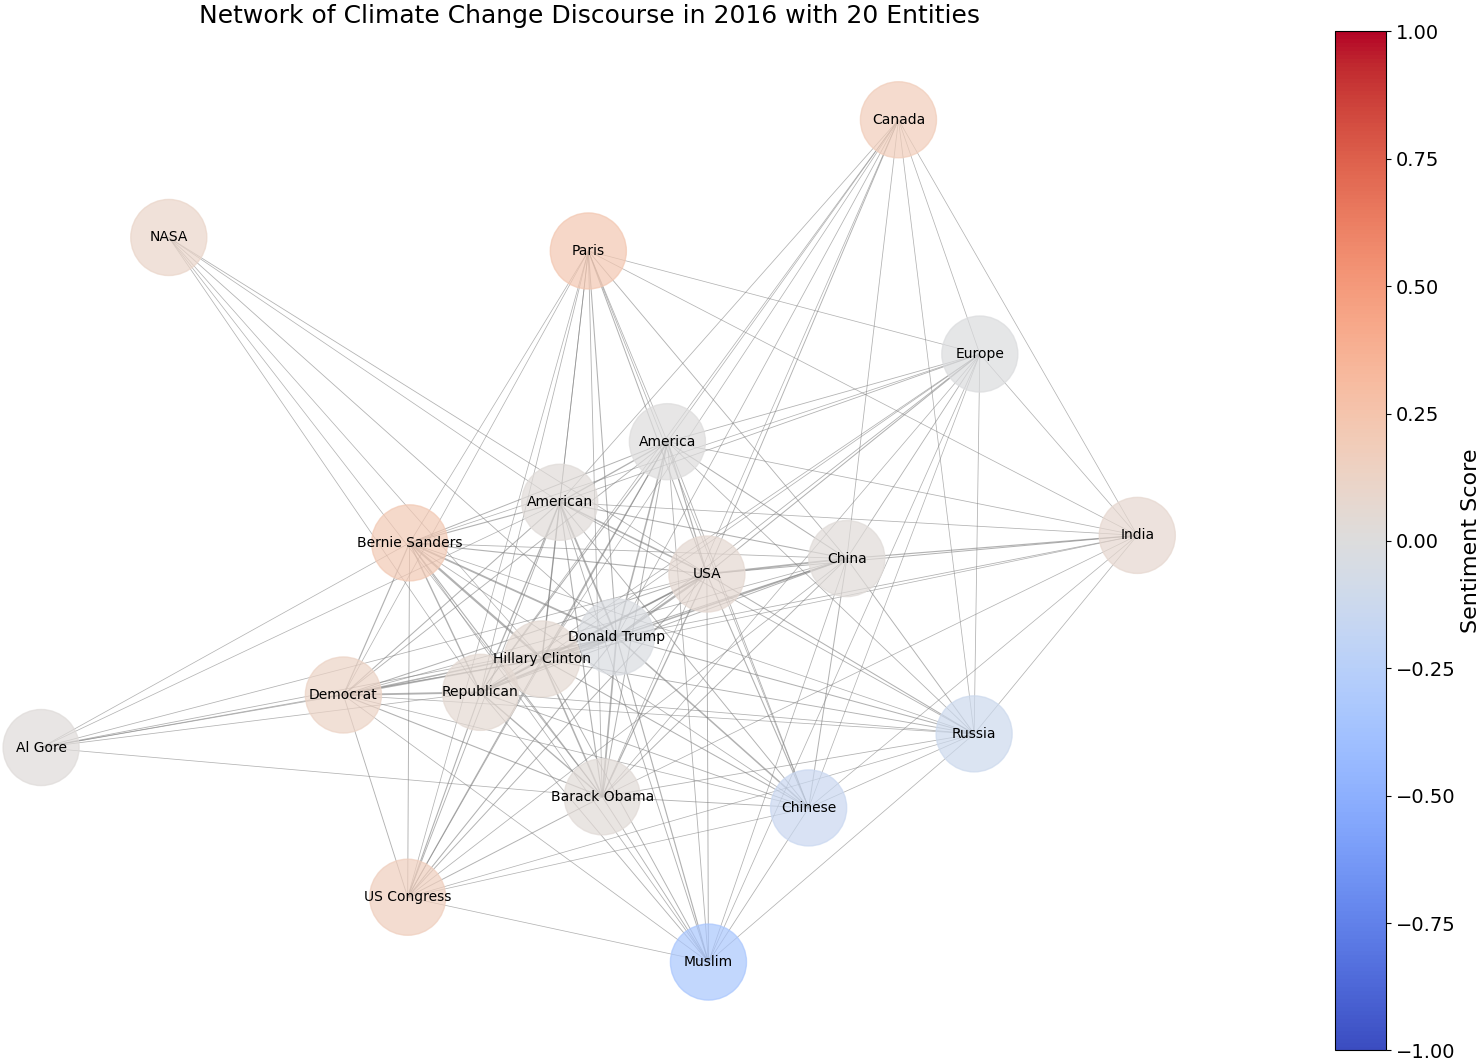
\includegraphics[width=\textwidth]{images/topic_details/entities/network_analysis_top20_2016_spring.png}
    \caption{Network of 20 Most Frequent Entities and their Sentiment in 2016}
    \label{fig:network_2016}
\end{figure}
In 2016, the network (Figure \ref{fig:network_2016}) shows a significant shift due to the US presidential election. Entities like Donald Trump, Hillary Clinton, and Bernie Sanders dominate the discourse, alongside traditional entities like the US Congress and NASA. The sentiment analysis reveals a mix of positive and negative sentiments, particularly around the election candidates, indicating polarized opinions.

\begin{description}
    \item[Democratic and Republican Candidates:] The main political figures were \emph{Donald Trump} (Republican) and \emph{Hillary Clinton} (Democrat), with Donald Trump ultimately winning the presidency despite having a lower sentiment score than Hillary Clinton. This difference may reflect the disputable nature of the election and the polarizing views on Trump's climate policies. Trump's rhetoric often focused on economic concerns over environmental regulations, which resonated with a significant portion of the voters despite generating negative sentiment in climate change discussions \cite{bbc2016trump}.
    \item[Paris Agreement:] The inclusion of \emph{Paris} is linked to the Paris Agreement, a major international treaty on climate change adopted in 2015. This agreement aimed to limit global warming and was a significant topic in climate discussions \cite{UN2019}.
    \item[Muslim Entity:] The very negative sentiment around \emph{Muslim} likely stems from the political rhetoric and policies of the time, including Trump's proposed travel ban and broader discussions around immigration and security. Trump's campaign included significant anti-immigration rhetoric, particularly targeting Muslim-majority countries, which contributed to the negative sentiment \cite{Gottfried_2023}.
    \item[Russia and Chinese Entities:] The negative sentiment around \emph{Russia} and  \emph{Chinese} could be related to discussions on international politics, cybersecurity concerns, and trade issues, all of which were prominent in 2016. Russia, often viewed negatively due to its geopolitical actions, including involvement in the Syrian Civil War and claims of interference in the US elections, likely contributed to this sentiment. The long-standing historical tensions from the Cold War also play a role in Russia's negative sentiment \cite{Ziegler2018}. For China, Trump's campaign rhetoric frequently criticized China's trade practices and accused China of currency manipulation, which fueled negative sentiments. These trade tensions and accusations of environmental irresponsibility by China in global forums added to the negative perception \cite{Steinbock2018}.
\end{description}

\subsubsection{2020 Network Analysis}
\begin{figure}[h]
    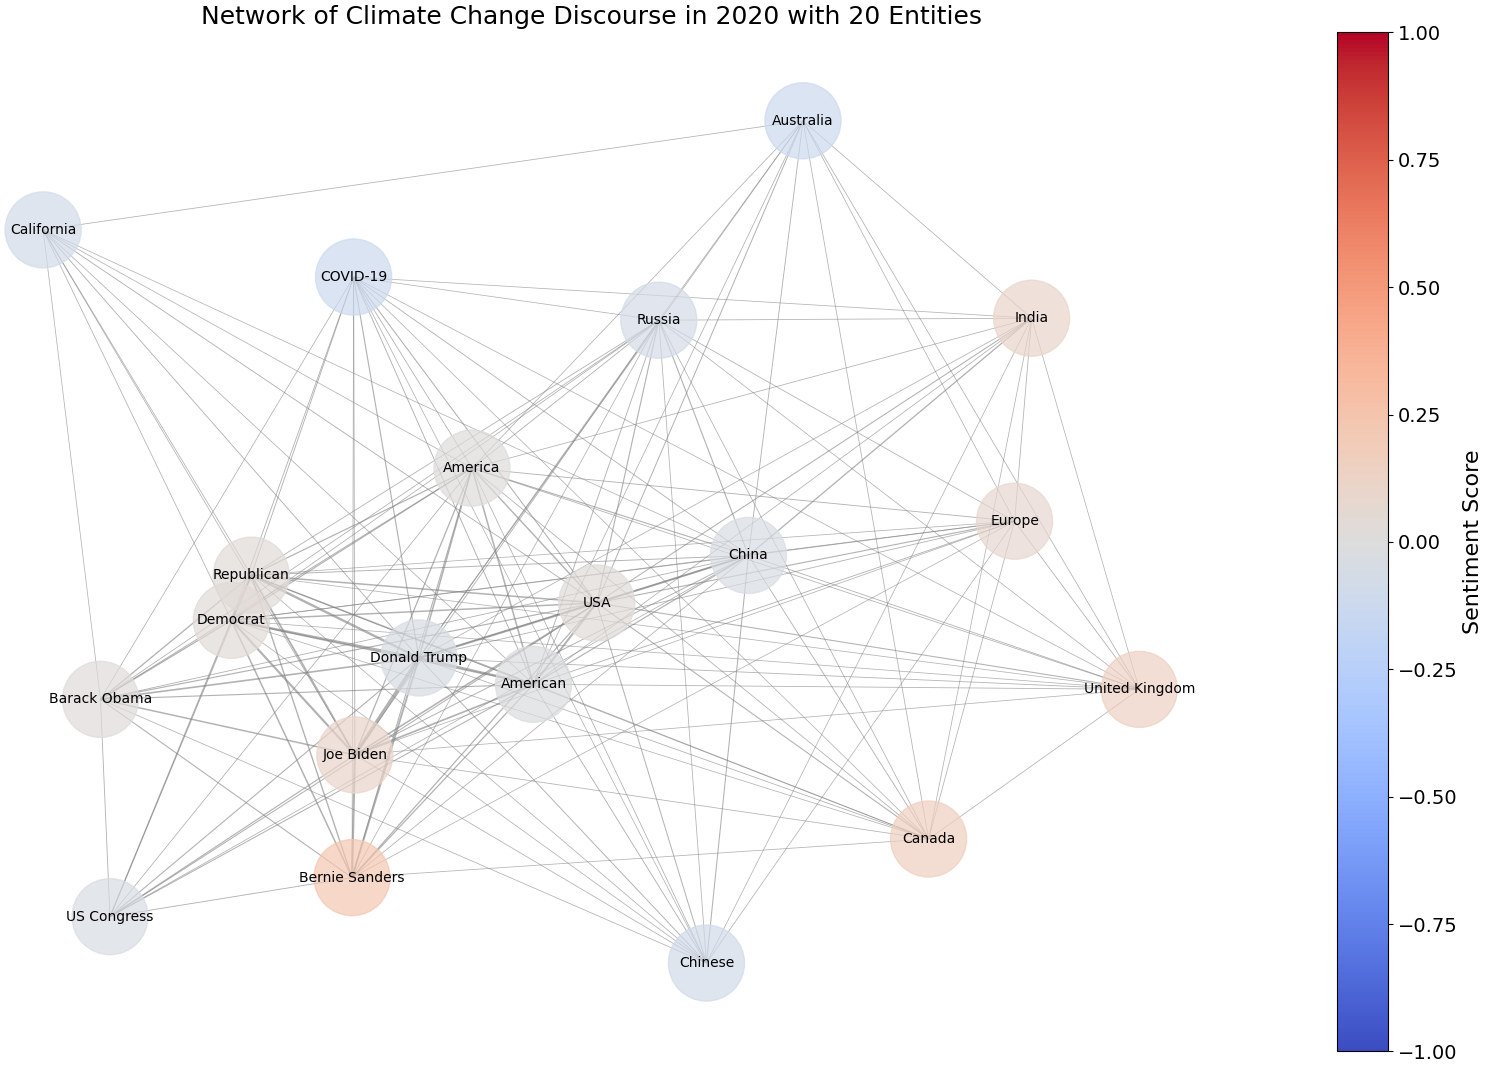
\includegraphics[width=\textwidth]{images/topic_details/entities/network_analysis_top20_2020_spring.png}
    \caption{Network of 20 Most Frequent Entities and their Sentiment in 2020}
    \label{fig:network_2020}
\end{figure}
The 2020 network graph presented in Figure \ref{fig:network_2020} is heavily influenced by the COVID-19 pandemic, with entities like \emph{COVID-19} and \emph{California} becoming prominent. The sentiment scores are more varied, reflecting the complex and diverse discussions around climate change during the pandemic. Political figures such as Donald Trump and Joe Biden are central, highlighting the impact of the US presidential election on climate change discourse.

\begin{description}
    \item[Democratic and Republican Candidates:] The key political figures in the 2020 election were \emph{Donald Trump} (Republican) and \emph{Joe Biden} (Democrat), with Joe Biden winning the presidency.
    \item[COVID-19 Pandemic:] The presence of \emph{COVID-19} reflects its global impact on all aspects of life, including environmental and climate policies. The pandemic led to discussions on how to build back better with greener policies. The significant reduction in industrial activity and transportation during the pandemic resulted in temporary decreases in carbon emissions and improved air quality in many regions. This situation highlighted the potential benefits of reducing emissions and stimulated conversations about sustainable recovery plans that integrate climate goals into economic recovery strategies \cite{JABAREEN2013220}. For instance, the water in Venice became clearer, and fish returned due to reduced boat traffic and pollution. Additionally, smog in some cities in China was significantly reduced, improving sight distance and air quality \cite{Xu_2020}. Moreover, the pandemic underscored the interconnections of global health and environmental sustainability, emphasizing the need for resilient and adaptive climate policies in the face of future crises \cite{interdisciplinary2021}.
    \item[Negative Sentiments:] Entities like \emph{Australia}, \emph{California}, \emph{Chinese}, and \emph{Russia} show negative sentiments similar to \emph{COVID-19}. This could be due to climate disasters like the Australian bushfires and California wildfires, as well as geopolitical tensions involving China and Russia. The rising conflict between Russia and Ukraine, which began escalating in 2014 and continued to burden international relations, also contributed to the negative sentiment towards Russia \cite{crisisgroup2022donbas}. Conflicts with China included trade wars initiated by Trump's administration, which heightened negative perceptions \cite{doi:10.1177/17480485231206364}.
    \item[Bernie Sanders and Canada:] \emph{Bernie Sanders} has the most positive sentiment, followed by \emph{Canada}. Sanders' progressive climate policies likely contributed to his positive sentiment. His proposals included the Green New Deal, which aimed to transition the US to 100\% renewable energy and create millions of jobs in the process \cite{sanders2020green}. Canada's environmental initiatives, such as carbon pricing, investment in green technology, and strong commitments to the Paris Agreement, have also obtained positive sentiment \cite{canada2020climate}.
\end{description}

The network analysis of climate change discourse on Reddit reveals a complex interplay of political, scientific, and global entities. The sentiment scores add a layer of understanding to how these entities are perceived, highlighting the importance of both political leadership and scientific expertise in the public discourse on climate change. This approach, using entity recognition and sentiment analysis, provides a more differentiated view of climate change discussions compared to simple n-gram analysis.

\section{Analysis of Organizational Mentions and Industrial Companies}
The analysis of frequently mentioned organizations in climate change discussions on Reddit reveals several notable trends and entities. The bar plot for 2013 (Figure \ref{fig:org_2013}) presents the frequency (absolute values are provided within the bar) and sentiment of the 15 most mentioned organizations, highlighting a strong U.S.-centric focus influenced by political and industrial contexts. This example provides an overview that helps move to analyzing the sentiment and frequency of specific U.S. companies over a broader time frame.

\begin{figure}[h]
    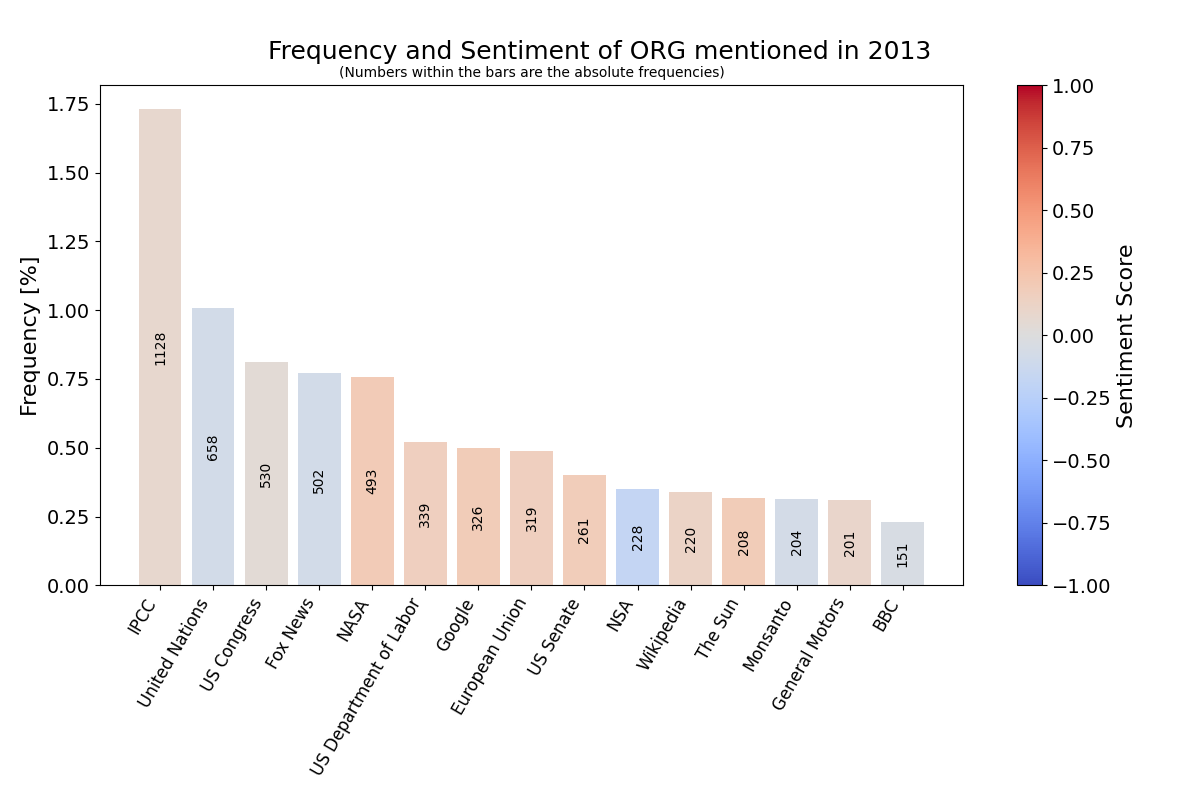
\includegraphics[width=\textwidth]{images/topic_details/entities/ORG_2013.png}
    \caption{Top 15 Most Frequent ORG Entities in 2013 with their Sentiments}
    \label{fig:org_2013}
\end{figure}

\subsection{Overview of Key Organizations in 2013}
\begin{description}
    \item[IPCC (Intergovernmental Panel on Climate Change)] The IPCC is the most frequently mentioned organization, reflecting its critical role in providing scientific assessments on climate change. With 1,128 mentions, it holds a positive sentiment score, underscoring its credibility and the reliance on its reports for climate policy and advocacy discussions. The IPCC's influence in 2013 was significant, with the release of the Fifth Assessment Report (AR5), which provided comprehensive evaluations of the physical science basis of climate change, impacts, adaptation, vulnerability, and mitigation strategies \cite{ipcc2013}.
    \item[NSA (National Security Agency)] The NSA exhibits the most negative sentiment among the listed organizations. This negative perception is likely influenced by the Edward Snowden reveals in 2013, which exposed widespread monitoring practices and triggered global debates on privacy and ethics. The  information shared by Snowden had far-reaching implications, leading to discussions about government control and civil liberties, which negatively impacted the public perception of the NSA \cite{lanchester2013}.
    \item[Monsanto] The negative sentiment towards Monsanto can be attributed to the "March Against Monsanto" protests in 2013. These protests highlighted public concerns over genetically modified organisms (GMOs) and pesticide use. The widespread demonstrations reflected the growing anxiety about Monsanto's practices and their potential impact on health and the environment \cite{guardian2013}.
\end{description}

Overall, the data from 2013 emphasize the intersection of climate change discourse with significant political and social events, highlighting the
connected nature of climate change and global governance. This U.S.-centric focus is evident from the dominance of entities related to U.S. politics and industries.

This example of 2013 leads us to a broader examination of the frequency and sentiment of specific U.S. companies, such as Amazon, Google, ExxonMobil, and Tesla. Understanding the role of these industrial giants is crucial, as they significantly influence and are influenced by climate change policies and public perception. Analyzing these companies helps to highlight the important connection between industrial activities and climate change discussions, revealing how public sentiment towards these corporations evolves over time. Industrial companies are generally important to understand, influence, and discuss climate change discourses due to their significant environmental impacts and roles in shaping sustainability practices.

\subsection{Analysis of Key U.S. Companies}
\subsubsection{Amazon}
\begin{figure}[h]
    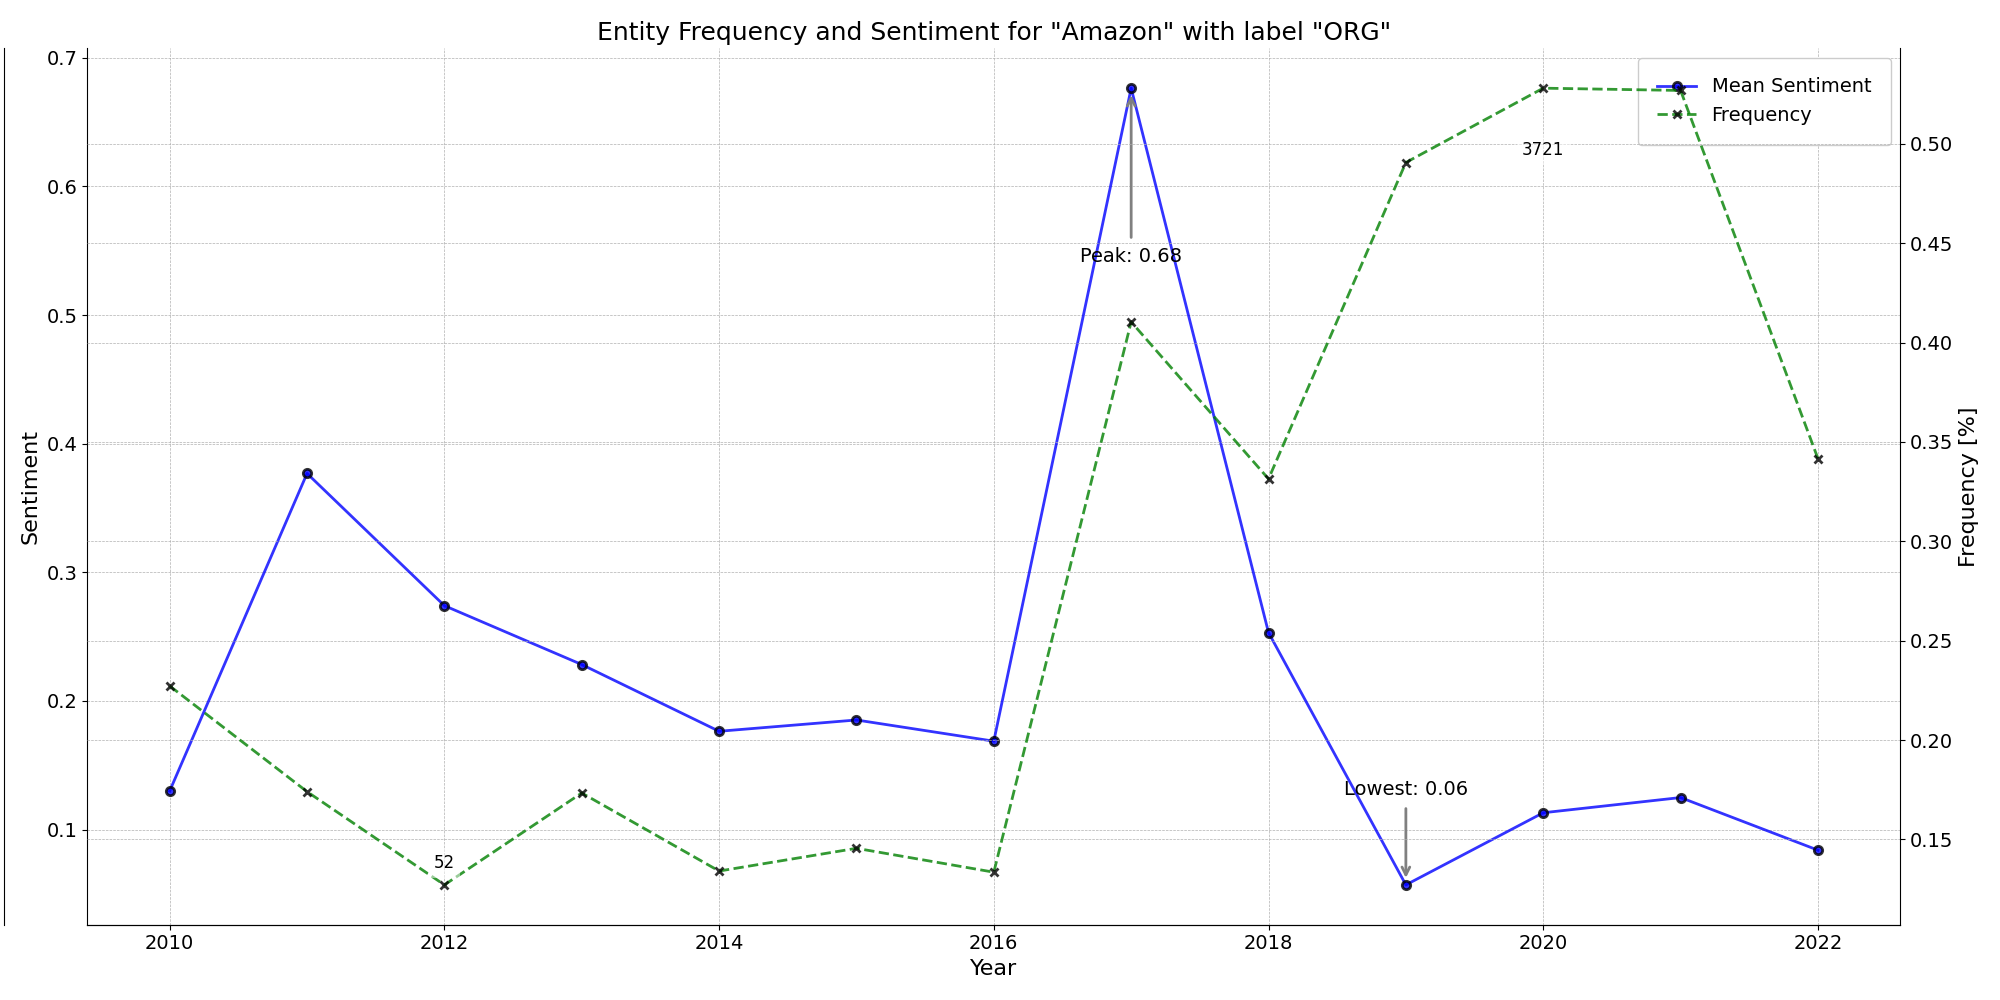
\includegraphics[width=\textwidth]{images/topic_details/entities/entity_frequency_Amazon.png}
    \caption{Trends in Amazon's Frequency and Sentiment in the Reddit Dataset}
    \label{fig:entity_amazon}
\end{figure}

Amazon is an American multinational technology company known for its e-commerce platform, cloud computing services, digital streaming, and artificial intelligence. Founded by Jeff Bezos in 1994, Amazon started as an online bookstore and quickly expanded into various other product categories. It is now one of the largest online retailers globally. The company also provides cloud computing services through Amazon Web Services (AWS), which has become a major player in the industry \cite{techtarget2024}.

Amazon shows a significant peak in frequency and sentiment in 2017, with a rapid drop in sentiment to an all-time low in 2019, followed by fluctuating trends in following years.

\begin{itemize}
    \item \textbf{2017 Peak:} The peak in 2017 corresponds to Amazon's initiatives in renewable energy investments and its commitment to sustainability, which positively impacted public sentiment \cite{amazon2017,ventura2017}.
    \item \textbf{2019 Decline:} The sharp drop in sentiment in 2019 can be linked to criticisms of Amazon's environmental practices and labor conditions. Employees staged a walkout demanding better climate policies, which negatively influenced public perception \cite{seattletimes2019}.
    \item \textbf{2020 Frequency Peak:} The highest frequency in 2020 is likely due to the COVID-19 pandemic, which increased Amazon's visibility and discussions around its operations and environmental impact. The rise in e-commerce during the pandemic brought attention to Amazon's carbon footprint and sustainability efforts \cite{moorhead2021amazon}.
\end{itemize}

\subsubsection{Google}
\begin{figure}[h]
    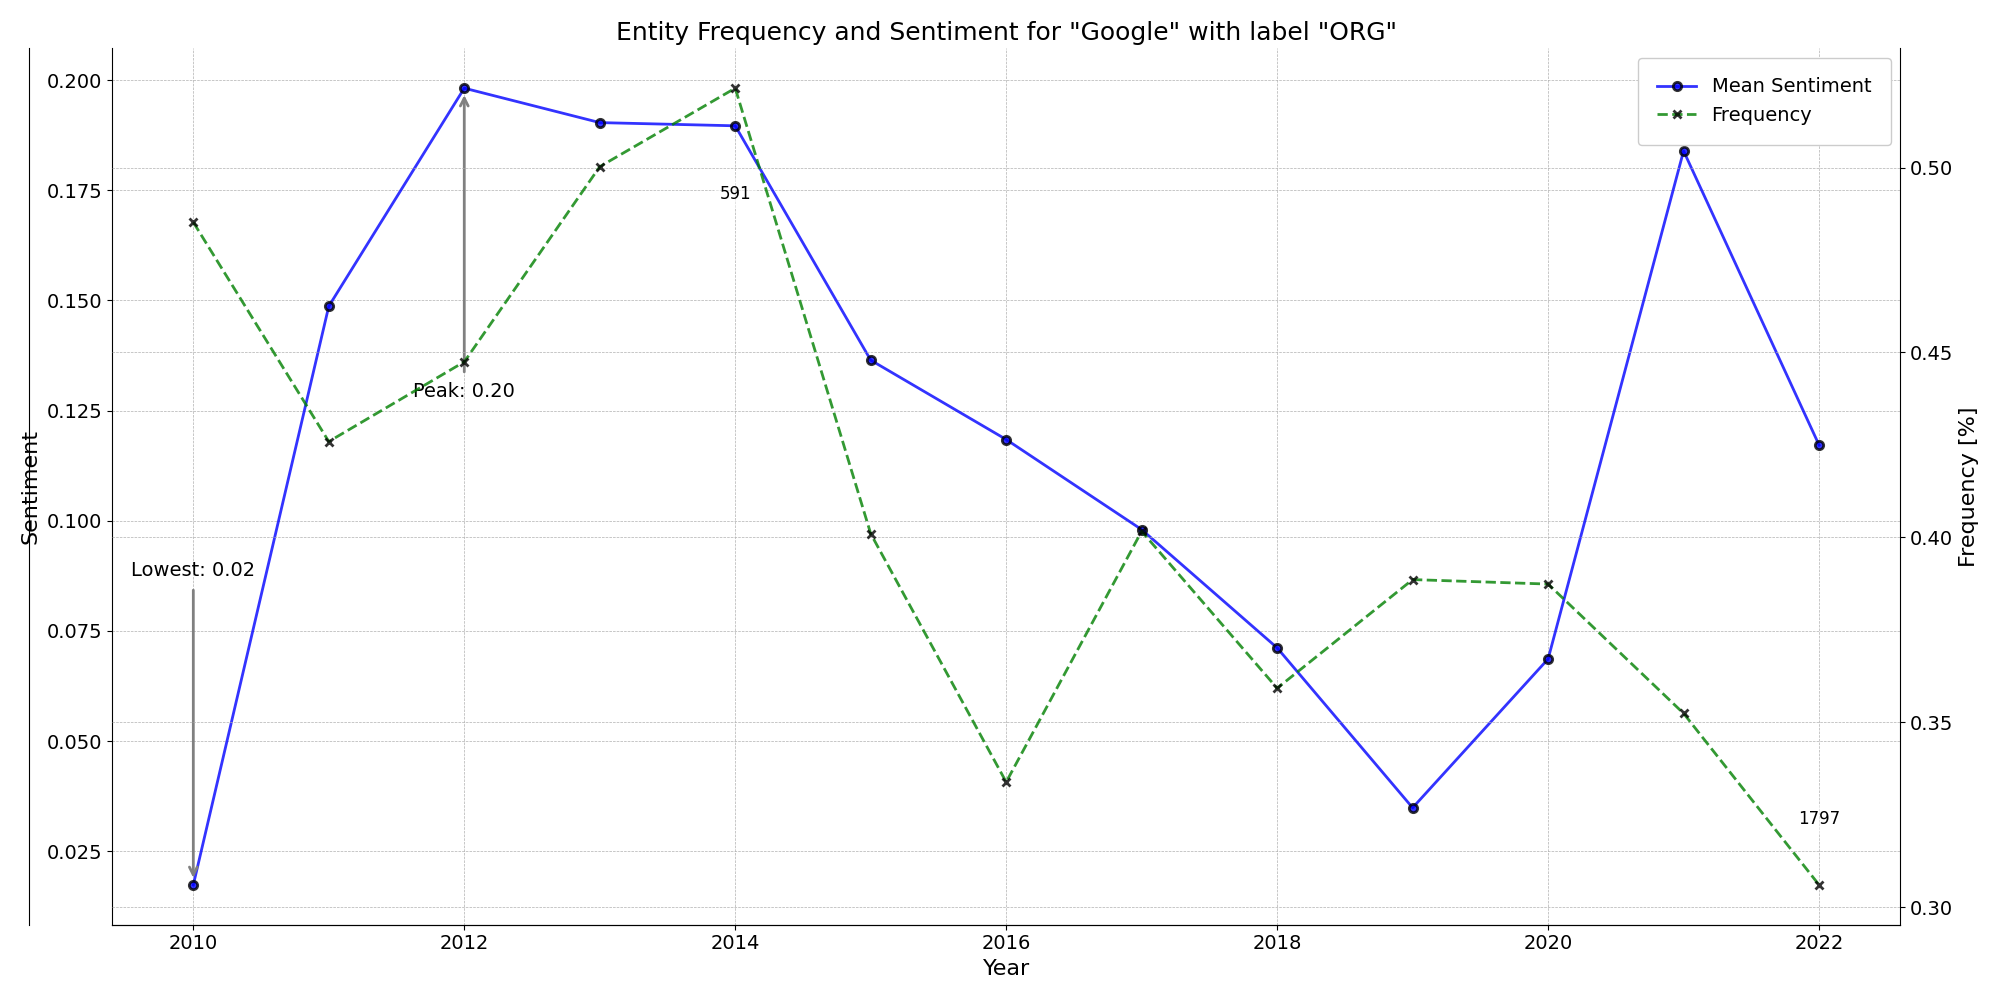
\includegraphics[width=\textwidth]{images/topic_details/entities/entity_frequency_Google.png}
    \caption{Trends in Google's Frequency and Sentiment in the Reddit Dataset}
    \label{fig:entity_google}
\end{figure}

Google, founded by Larry Page and Sergey Brin in 1998, is a leading technology company known for its search engine, advertising services, and numerous digital products such as Gmail, Google Maps, and YouTube. It operates under its parent company, Alphabet Inc., and has made significant investments in artificial intelligence, renewable energy, and autonomous driving technologies \cite{britannica2024}.

Google shows a progression from a neutral sentiment in 2010 to a peak in 2013, followed by a drop and a regrowth in 2020 and 2021.

\begin{itemize}
    \item \textbf{2012-2013 Increase:} The significant rise in sentiment during these years is due to Google's significant investments in renewable energy projects and its commitment to carbon neutrality. These efforts were well-received and highlighted Google's leadership in green technology \cite{wemeanbusiness2024,google2013}.
    \item \textbf{Subsequent Decline:} The gradual drop in sentiment might reflect growing close inspection of tech companies' environmental footprints and broader societal impacts. Issues like data privacy and corporate influence may have contributed to the mixed sentiments \cite{PENZ20181125}.
    \item \textbf{2020-2021 Resurgence:} The resurgence in positive sentiment aligns with Google's continued leadership in sustainability initiatives and advancements in green technology. Their efforts to reduce carbon emissions and promote renewable energy use have strengthened their reputation \cite{fastcompany2016}.
\end{itemize}

\subsubsection{ExxonMobile}
\begin{figure}[h]
    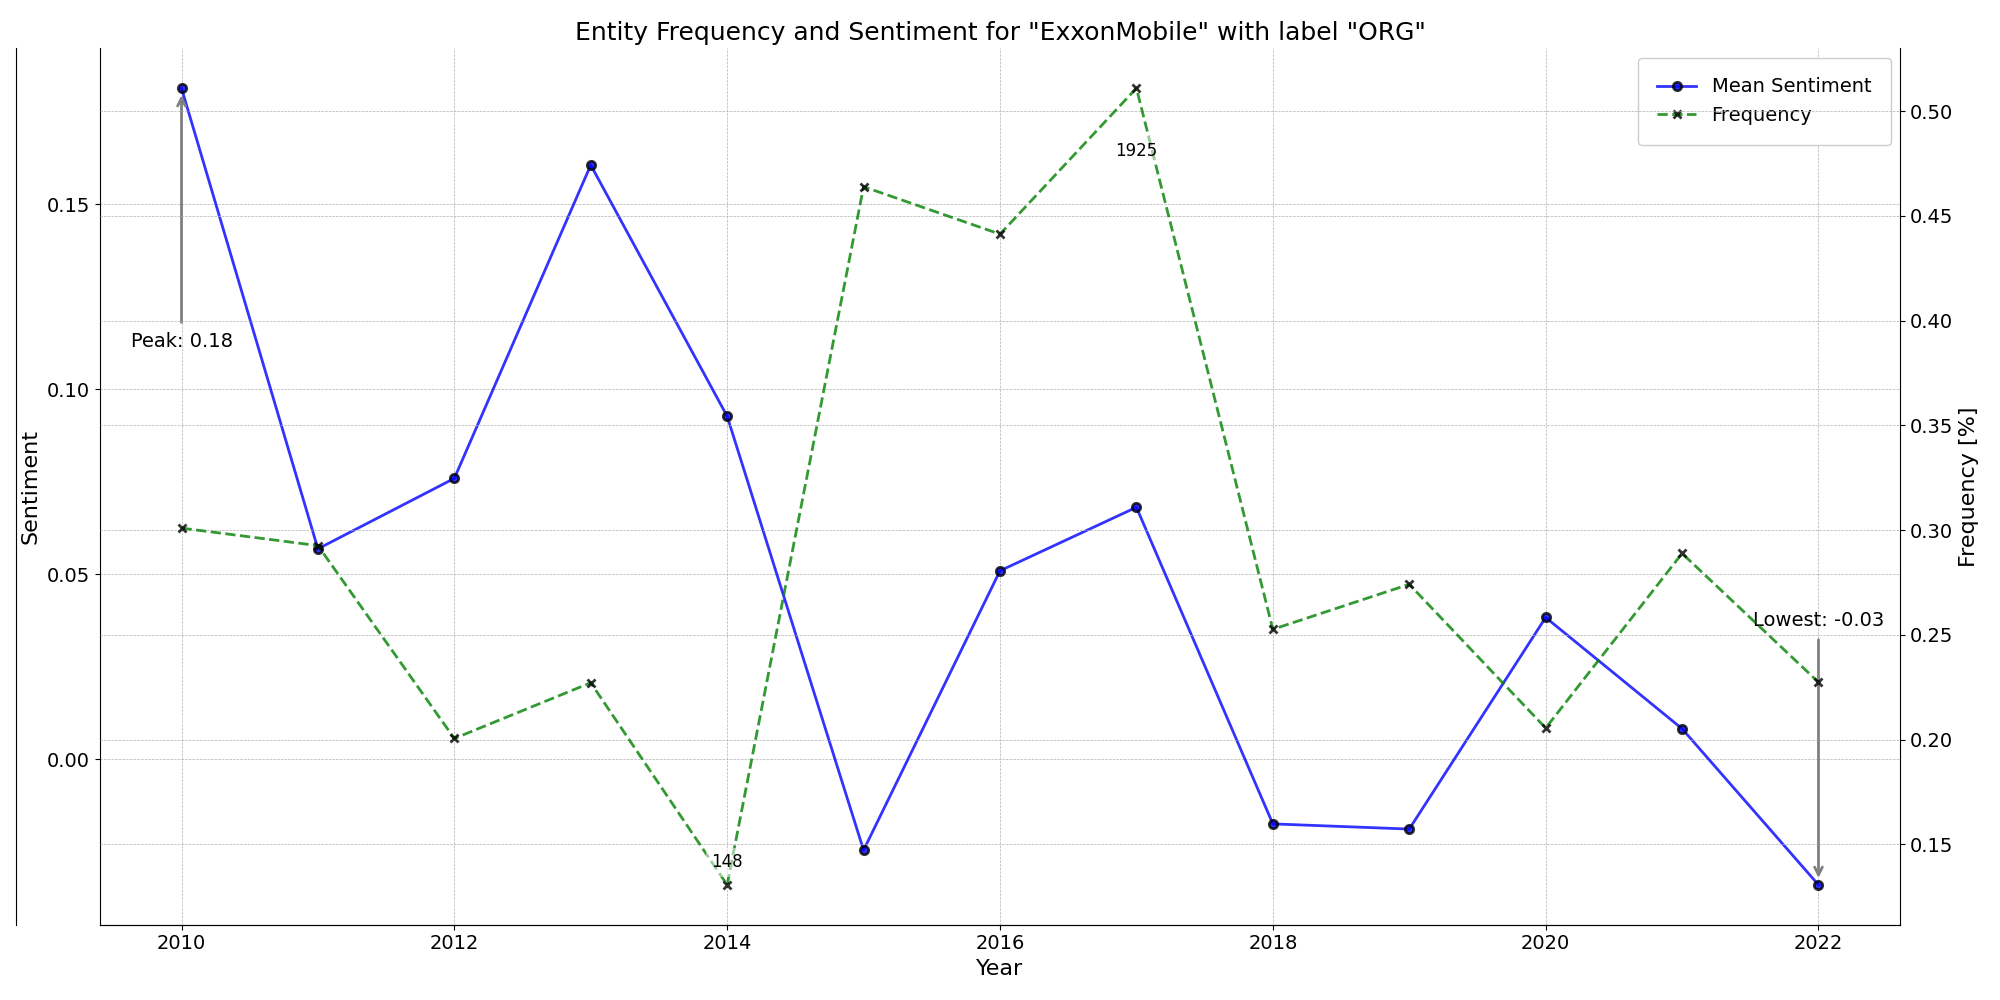
\includegraphics[width=\textwidth]{images/topic_details/entities/entity_frequency_ExxonMobile.png}
    \caption{Trends in ExxonMobil's Frequency and Sentiment in the Reddit Dataset}
    \label{fig:entity_exxonmobile}
\end{figure}

ExxonMobil is one of the world's largest publicly traded oil and gas companies, formed in 1999 through the merger of Exxon and Mobil. It is known for its widespread operations in oil exploration, production, refining, and marketing. ExxonMobil has faced criticism for its role in contributing to climate change and its historical stance on climate science \cite{worldbank2024,britannica2024exxon}.

ExxonMobil shows the highest frequencies from 2014 to 2016, with generally decreasing sentiment, nearing negative territory by 2022.

\begin{itemize}
    \item \textbf{2014-2016 High Frequencies:} These years marked intense discussions around fossil fuels and climate policies, influenced by the Obama administration's environmental regulations and global oil market dynamics. The Keystone XL pipeline debates and the Paris Agreement also played a role in increasing mentions \cite{worldbank2024,climatechangenews2015}.
    \item \textbf{2013 Sentiment Peak:} The peak in sentiment in 2013 could be attributed to ExxonMobil's public statements on reducing greenhouse gas emissions and investments in clean energy, although these claims often faced skepticism \cite{spiegel2017}.
    \item \textbf{2022 Low:} The drop to near-negative sentiment in 2022 reflects ongoing criticisms of ExxonMobil's environmental record and recognized greenwashing. Public and regulatory pressures have increased examination on fossil fuel companies \cite{plosone2024}.
\end{itemize}

\subsubsection{Tesla}
\begin{figure}[h]
    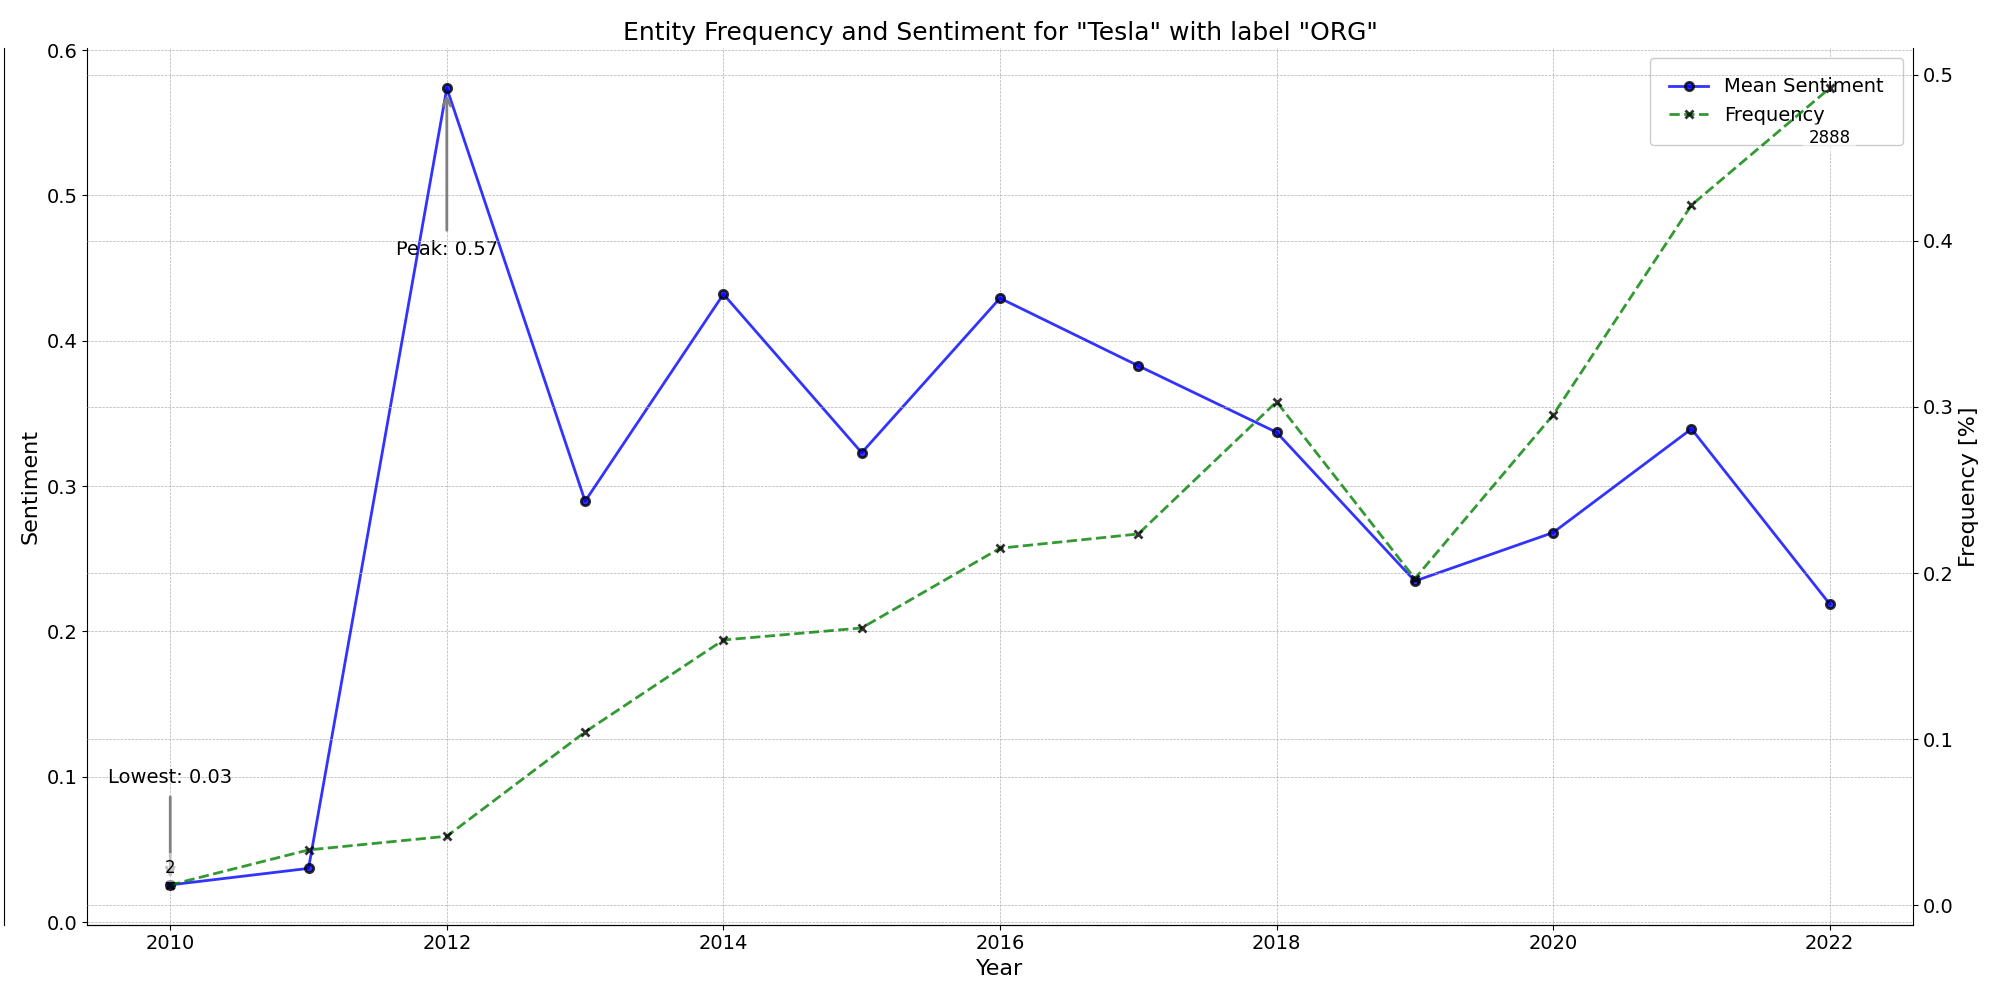
\includegraphics[width=\textwidth]{images/topic_details/entities/entity_frequency_Tesla.png}
    \caption{Trends in Tesla's Frequency and Sentiment in the Reddit Dataset}
    \label{fig:entity_tesla}
\end{figure}

Tesla, founded by Elon Musk, Martin Eberhard, Marc Tarpenning, JB Straubel, and Ian Wright in 2003, is known for its electric vehicles (EVs), energy storage solutions, and solar products. Tesla has revolutionized the automotive industry with its high-performance EVs and has been a leader in promoting sustainable energy solutions \cite{britannica2024tesla}.

Tesla exhibits a stable increase in frequency over the years, peaking in 2022. Sentiment peaked significantly in 2012, with a stable trend and slight decrease afterward.

\begin{itemize}
    \item \textbf{2012 Sentiment Peak:} The peak in sentiment in 2012 is linked to Tesla's Model S release, which revolutionized the electric vehicle market and received widespread praise. This innovation positioned Tesla as a leader in sustainable transportation \cite{tesla2012,teslamag2022}.
    \item \textbf{Stable Frequency Increase:} Tesla's frequency rise reflects its growing influence in the clean energy and automotive sectors, aligning with increased public and media attention. Tesla's innovations in battery technology and renewable energy solutions contribute to its prominence in climate change discussions.
    \item \textbf{2022 Frequency Peak:} The peak in 2022 coincides with Tesla's expanded market presence and ongoing innovations. The company's advancements in electric vehicles and energy storage solutions have kept it at the forefront of discussions about sustainable technology \cite{notateslaapp2023}.
\end{itemize}

\section{Analysis of Frequency and Sentiment of US Presidents}
\begin{figure}[h]
    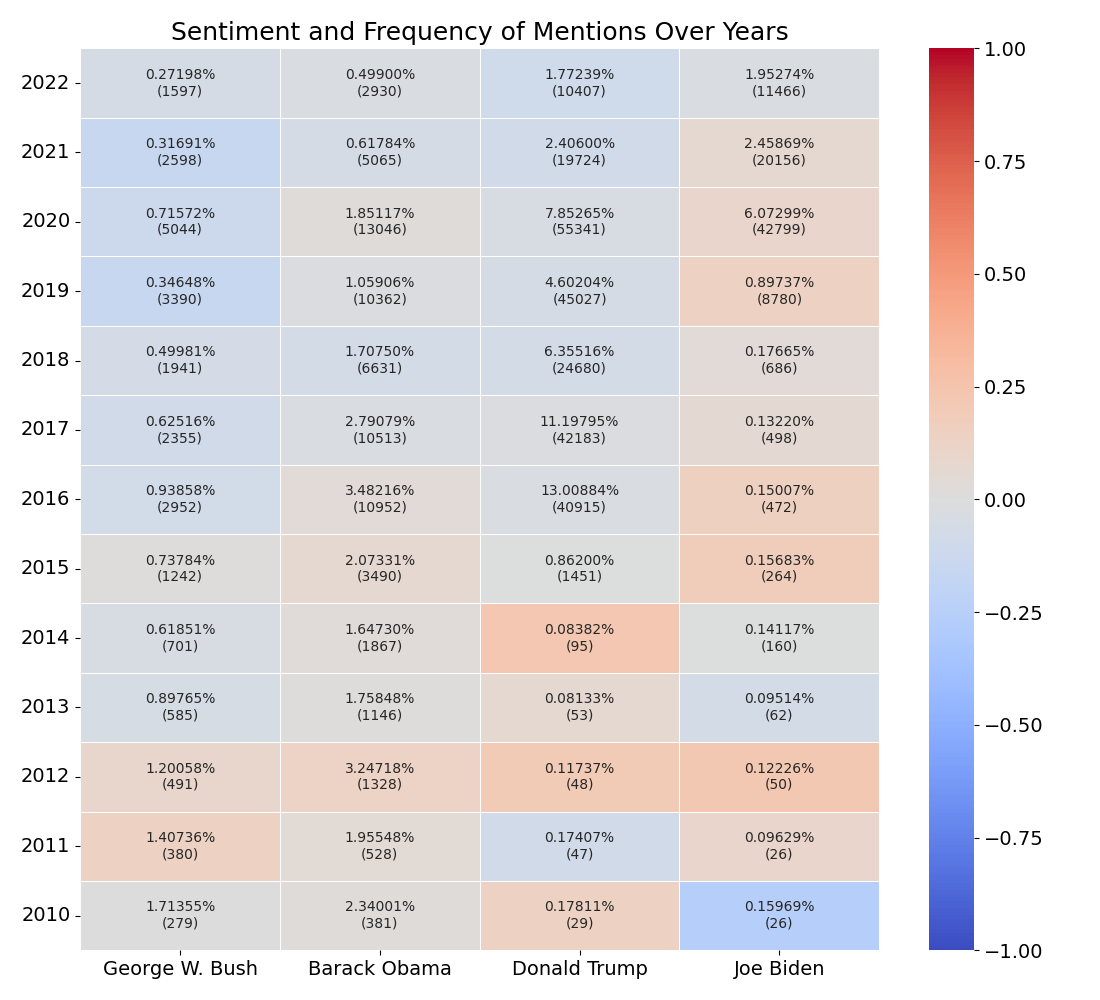
\includegraphics[width=\textwidth]{images/topic_details/entities/heatmap_sentiment_and_frequency_4entities_PERSON.png}
    \caption{Heatmap of US Presidents' Frequency and Sentiment in the Reddit Dataset}
    \label{fig:president_entities}
\end{figure}

The heatmap provided in Figure \ref{fig:president_entities} illustrates the sentiment and frequency of mentions for four US Presidents (George W. Bush, Barack Obama, Donald Trump, and Joe Biden) from 2010 to 2022. This analysis explores the patterns observed in the data, focusing on peaks and drops in both frequency and sentiment.
The dataset covers the period from 2010 to 2022 and includes mentions of four US Presidents:

\begin{itemize}
    \item \textbf{George W. Bush:} Although his presidency ended in 2009, he remains part of the discourse, particularly in relation to his climate policies \cite{Meyer2023}.
    \item \textbf{Barack Obama:} President from 2009 to 2017, with a continued presence in the climate change discussion post-presidency \cite{obamaclimatechangerecord}.
    \item \textbf{Donald Trump:} President from 2017 to 2021, who remains a significant figure in climate change discourse even after his term ended \cite{bbc2020trump}.
    \item \textbf{Joe Biden:} Elected in 2020 and currently serving as president, showing a notable presence in recent years \cite{wri2022biden}.
\end{itemize}

Election years show significant peaks in mentions for the presidents involved in the campaigns. For instance, 2016 shows a substantial increase in mentions for Donald Trump as he ran for and was elected president. Similarly, in 2020, both Donald Trump and Joe Biden show peaks in mentions due to their participation in the presidential election. These peaks highlight the heightened public and media attention during election periods.

Even after their terms, presidents maintain a presence in climate change discourse. George W. Bush continues to be mentioned, although his frequency decreases over time. Barack Obama remains consistently mentioned, reflecting ongoing discussions about his climate policies and initiatives. Donald Trump, in particular, maintains an unusually high frequency in mentions even after his presidency, especially in 2021 and 2022. This can be attributed to his polarizing climate policies, continued public statements, actions that keep him in the public eye, and his extensive use of social media to communicate with the public \cite{trumptruthsocial}. Joe Biden, as the current president, naturally has high mentions reflecting his active role in current climate policies.

George W. Bush's sentiment decreases over the years, indicating increasing skepticism toward his climate policies. This trend could be due to the long-term impacts of his administration's policies becoming more apparent over time. Barack Obama's sentiment remains relatively stable, suggesting a balanced view of his climate actions, with his efforts in the Paris Agreement and renewable energy investments being positively received. Donald Trump's sentiment shows a slight drop, reflecting controversies and criticisms surrounding his climate policies, such as exit from the Paris Agreement and promoting fossil fuels \cite{state2020,columbiaclimate2024}. However, the sentiment for Trump has notable peaks and drops, with 2014 and 2020 being outliers, likely due to fewer mentions causing fluctuation.

Joe Biden exhibits the most positive overall sentiment among the presidents during the data period. This could be attributed to his strong stance on climate change, rejoining the Paris Agreement, and ambitious climate policies like the Infrastructure Bill aimed at promoting clean energy and reducing emissions. His proactive approach and clear commitment to addressing climate issues resonate positively with the public and media.

Even after not being re-elected, Donald Trump continues to have a high frequency of mentions. This untypically high frequency is likely due to his continuous involvement in public debates, media coverage of his statements, ongoing influence within the political landscape, and his significant presence on social media platforms \cite{trumptruthsocial}. His controversial and often polarizing views on climate change ensure he remains a significant topic of discussion.

Joe Biden's positive sentiment reflects his clear and consistent climate policies, which align with scientific consensus and international efforts to fight climate change. His administration's efforts to reverse Trump's policies and reestablish environmental protections contribute to this positive perception \cite{grist2023}.

The decrease in sentiment for ex-presidents can be attributed to backdated evaluations of their policies. Once out of office, the long-term impacts of their decisions become clearer, often leading to more critical assessments. For example, George W. Bush's sentiment decline reflects ongoing skepticism about his administration's climate actions, while Donald Trump's decreasing sentiment post-presidency highlights continued debates surrounding his policies.

Overall, climate policy tends to be viewed more skeptically after a president's term ends. This backdated view allows for a more critical assessment of the effectiveness and consequences of their policies. The sentiment trends observed for George W. Bush and Donald Trump indicate that the public and media often re-evaluate the impacts of past administrations with a more critical viewpoint, leading to decreased sentiment over time.

This detailed analysis underscores the dynamic nature of public and media perception of US Presidents in the context of climate change. Election periods, ongoing public involvement, and backdated evaluations play significant roles in shaping both the frequency of mentions and the sentiment towards these leaders.